For the sentence segmentation we used the library spacy. Each category is displayed in figure 1. The x-axis is shows the length of a review in number of sentences, and the y-axis shows the total number of reviews of such length. 
	\begin{center}
		\begin{table}[!h]
			\caption{Average length of the sentences in the different star categories}
			\begin{tabular}{c | c | c | c | c}
				1 Star & 2 Star & 3 Star  & 4 Star & 5 Star\\\hline
				30.5 & 25.9 & 24.0  & 25 & 24\\
			\end{tabular}
		\end{table}
	\end{center}
	
	\begin{figure}
		\caption{Histograms of the length of the sentences}
		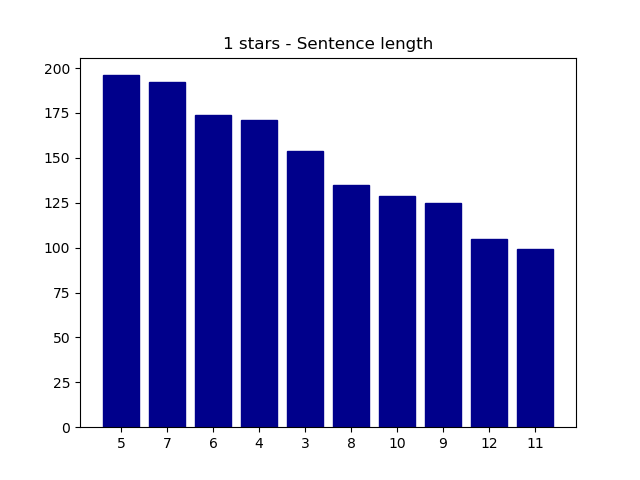
\includegraphics[scale=0.3]{figures/1stars-Sentencelength.png}
		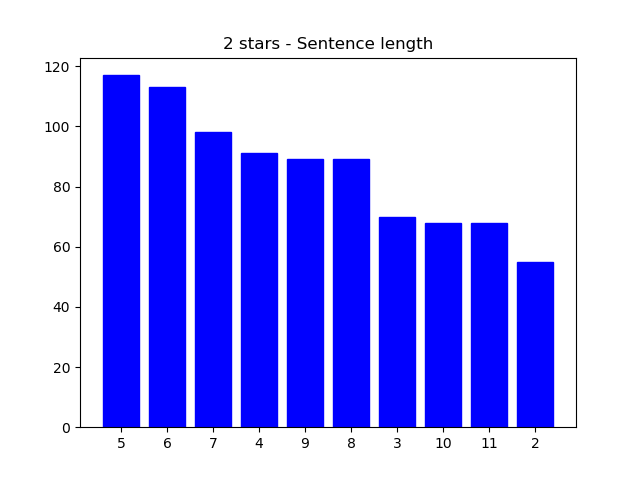
\includegraphics[scale=0.3]{figures/2stars-Sentencelength.png}
		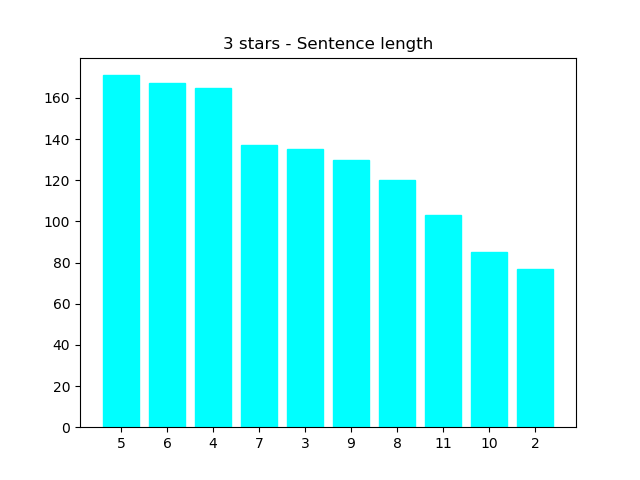
\includegraphics[scale=0.3]{figures/3stars-Sentencelength.png}
		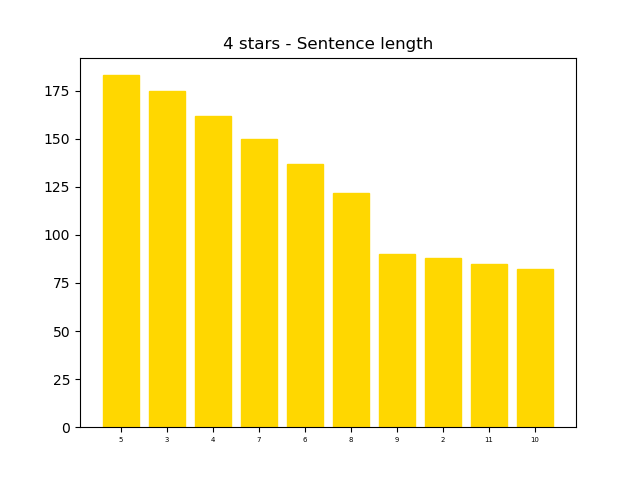
\includegraphics[scale=0.3]{figures/4stars-Sentencelength.png}
		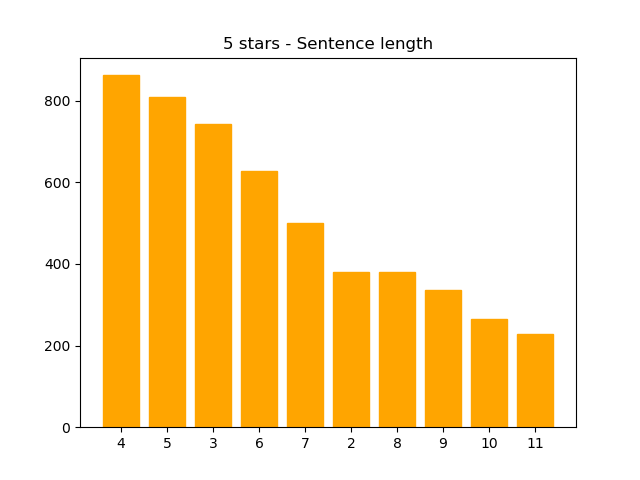
\includegraphics[scale=0.3]{figures/5stars-Sentencelength.png}
	\end{figure}
As can be seen, the length of the reviews are larger in bad ratings than in good ratings. This can also be seen in the average review length (Table 1). The average length of a review with a 1 star rating is 6 sentences larger than the average length of sentences of a review with 5 Stars. 
	